\documentclass[a4paper,12pt]{article}

%%% Работа с русским языком
\usepackage{cmap}					% поиск в PDF
\usepackage{mathtext} 				% русские буквы в формулах
\usepackage[T2A]{fontenc}			% кодировка
\usepackage[utf8]{inputenc}			% кодировка исходного текста
\usepackage[english,russian]{babel}	% локализация и переносы
\usepackage{xcolor}
\usepackage{hyperref}
 % Цвета для гиперссылок
\definecolor{linkcolor}{HTML}{799B03} % цвет ссылок
\definecolor{urlcolor}{HTML}{799B03} % цвет гиперссылок

\hypersetup{pdfstartview=FitH,  linkcolor=linkcolor,urlcolor=urlcolor, colorlinks=true}

%%% Дополнительная работа с математикой
\usepackage{amsfonts,amssymb,amsthm,mathtools} % AMS
\usepackage{amsmath}
\usepackage{icomma} % "Умная" запятая: $0,2$ --- число, $0, 2$ --- перечисление

%% Номера формул
%\mathtoolsset{showonlyrefs=true} % Показывать номера только у тех формул, на которые есть \eqref{} в тексте.

%% Шрифты
\usepackage{euscript}	 % Шрифт Евклид
\usepackage{mathrsfs} % Красивый матшрифт

%% Свои команды
\DeclareMathOperator{\sgn}{\mathop{sgn}}

%% Перенос знаков в формулах (по Львовскому)
\newcommand*{\hm}[1]{#1\nobreak\discretionary{}
{\hbox{$\mathsurround=0pt #1$}}{}}
% графика
\usepackage{graphicx}
\graphicspath{{pictures/}}
\DeclareGraphicsExtensions{.pdf,.png,.jpg}
\author{Бурмашев Григорий, БПМИ-208}
\title{ТВиМС, дз -- 8}
\date{\today}
\begin{document}
\maketitle
\section*{Номер 1}
Решим сначала отдельно для $x_q$, а потом для $y_q$, т.к вероятности различаются.

\begin{center}
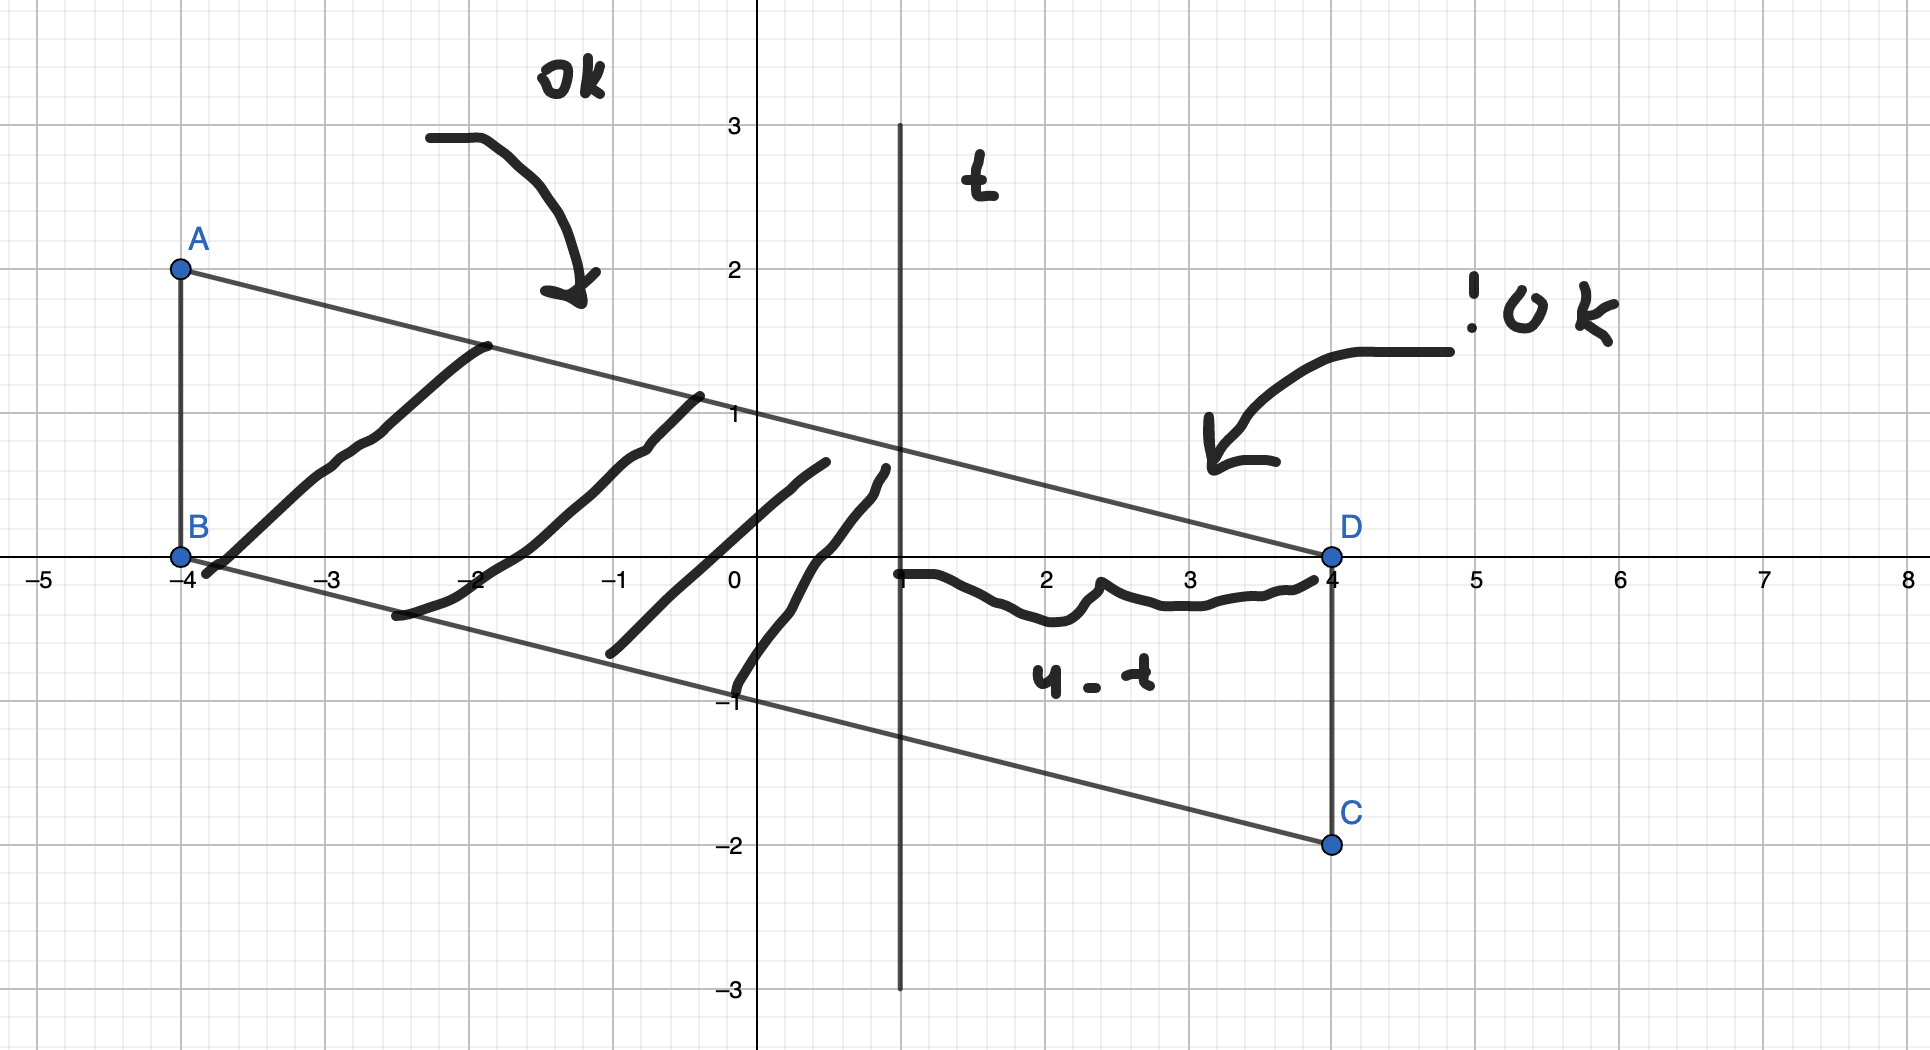
\includegraphics[scale=0.2]{1.png}
\end{center}
Разобьем на случаи, как обычно:
\begin{enumerate}
\item $t < -4$:

Очевидный случай
\[
P(x_q \leq t) = 0
\]
\item $ t \in [-4, 4)$:

Выберем точку $t$, все что справа от нее нам подходит, все что слева -- нет (в рамках нашего параллелограмма), т.к стороны одинаковые, влияет лишь высота, у правого будет $4 - t$, а высота всего параллелограмма $8$
\[
P(x_q \leq t) =  1 -  P(x_q > t)  = 1 - \frac{S{_{!ok}}}{S_{ABCD}} = 1 - \frac{4-t}{8} = \frac{t+4}{8}
\]
\item $ t \geq 4$:

Очевидный случай
\[
P(x_q \leq t) = 1 
\]
\end{enumerate}

Теперь решим для $y_q$  аналогичным образом:
\begin{center}

\includegraphics[scale=0.2]{2.png}
\end{center}
\begin{enumerate}
\item $t < -2$:

Очевидный случай
\[
P(y_q \leq t) = 0
\]

\item $t \in [0, 2)$:

Все аналогично ситуации с $x$, только теперь отделяем $t$ по оси $y$. Нам подходит все, что не попадет в верхний треугольник. Тогда нашу вероятность можно посчитать как 1 минус вероятность того, что попало в верхний треугольник. А она в свою очередь равна вероятности попасть в треугольник $ABD$ (а это ровно $\frac12$),  умноженной на отношение площадей верхнего треугольника к треугольнику $ABD$, т.е:
\[
P(y_q \leq t) = 1 - \frac{1}{2} \cdot \frac{S_{!ok}}{S_{ABD}} =  1 - \frac12 \cdot \left( \frac{h_{!ok}}{h_{ABD}} \right)^2 =  1 - \frac{1}{2} \cdot \left( \frac{2-t}{2} \right)^2 = 1 - \frac{(2-t)^2}{8}
\]

\item $t \in [-2, 0)$:

Задача зеркальная предыдущей, только теперь треугольник будет снизу, а мы хотим быть выше него, вероятность попасть в нижнюю часть параллелограмма также равна $\frac{1}{2}$, поэтому ответом будет просто дополнение предыдущей вероятности:
\[
P(y_q \leq t) =  \frac{(2-t)^2}{8}
\]
\item $t \geq 2$:

Очевидный случай
\[
P(y_q \leq t) = 1
\]
\end{enumerate}
\clearpage
\section*{Номер 2}
Для независимости по определению хотим $P(A \cap B) = P(A) \cdot P(B)$
\subsection*{a) $P(x_q \leq 1), P(y_q \leq 0)$}
\[
P(x_q \leq 1) = \frac{1 + 4}{8} = \frac{5}{8} 
\]
\[
P(y_q \leq 0) = \frac{1}{2}
\]
\[
P(x_q \leq 1) \cdot P(y_q \leq 0) = \frac{5}{8}\cdot \frac12 = \frac{5}{16}
\]
\begin{center}
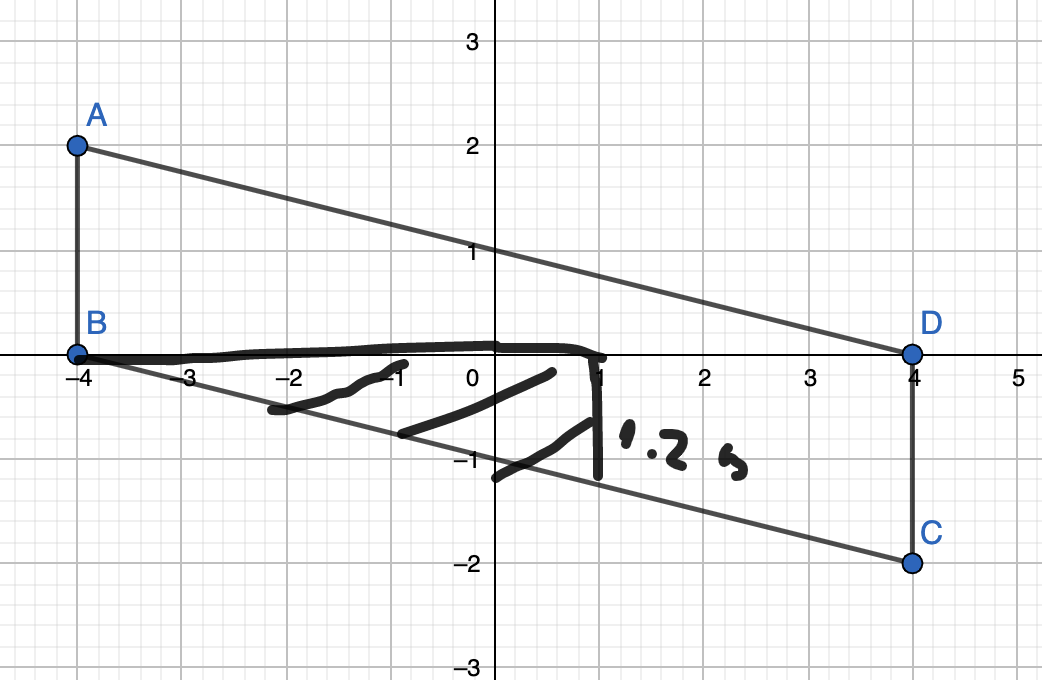
\includegraphics[scale=0.4]{3.png}
\end{center}
\[
P(x_q \leq 1 \cap y_q \leq 0) = \frac{S_{\text{треуг}}}{S_{ABCD}} = \frac{5 \cdot 1.25 \cdot \frac{1}{2}}{8 \cdot 2} = \frac{25}{128}
\]
\[
P(x_q \leq 1) \cdot P(y_q \leq 0) \neq P(x_q \leq 1 \cap y_q \leq 0)
\]
$\rightarrow$ \textbf{события зависимы}
\subsection*{b) $P(x_q \leq 0), P(y_q \leq \sqrt{2})$}
\[
P(x_q \leq 0) = \frac{1}{2}
\]
\[
P(y_q \leq \sqrt{2}) = 1 - \frac{(2 - \sqrt{2})^2}{8} = \frac{1}{4} \cdot (1 + 2\sqrt{2})
\]
\[
P(x_q \leq 0) \cdot P(y_q \leq \sqrt{2}) = \frac{1}{8} \cdot (1 + 2\sqrt{2})
\]
\begin{center}
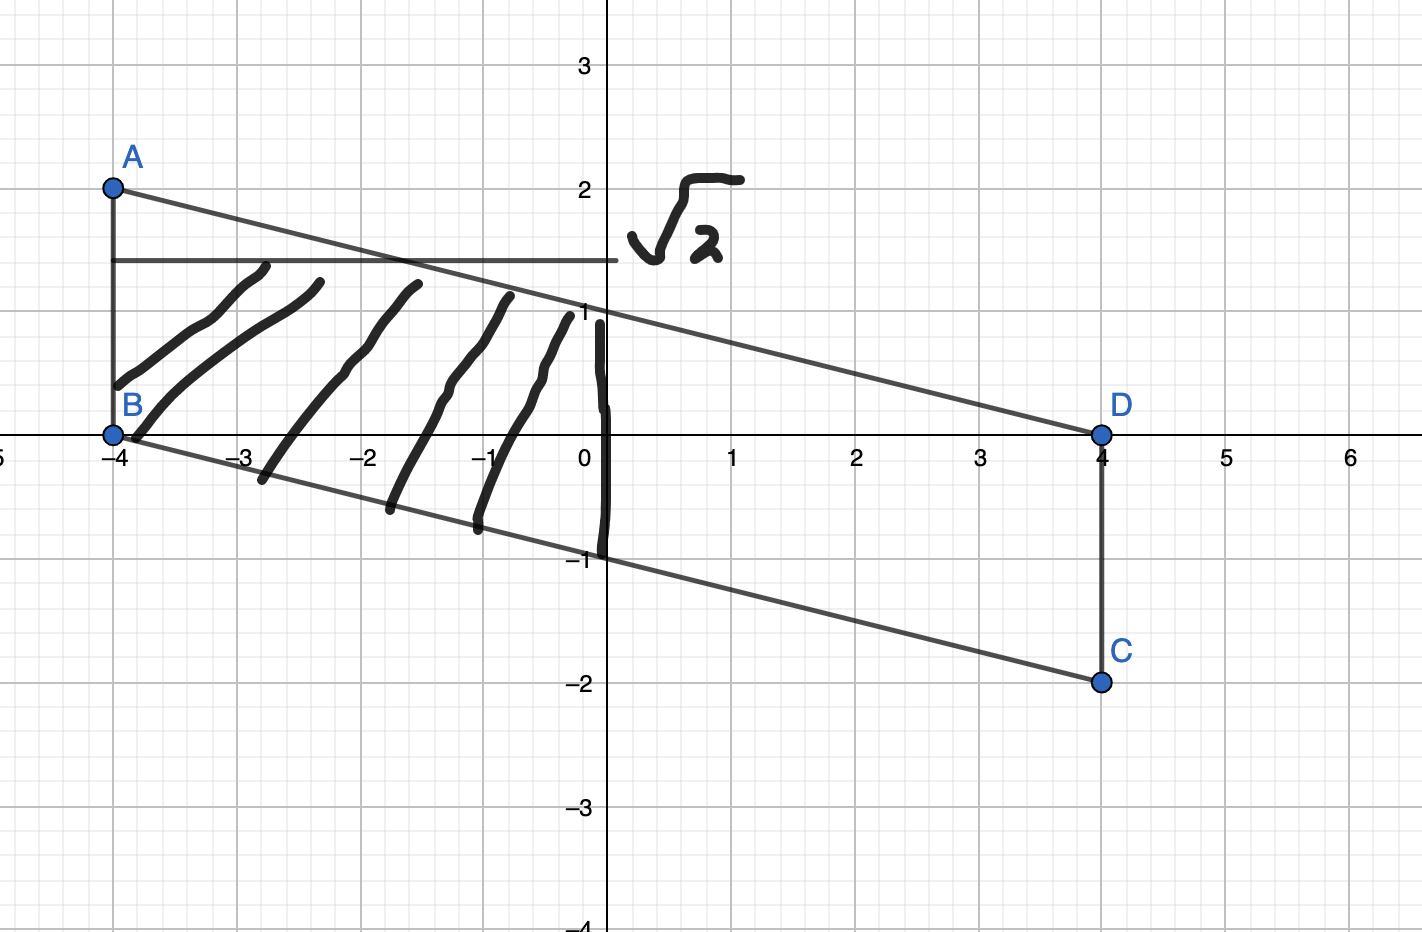
\includegraphics[scale=0.4]{4.png}
\end{center}
\[
P(x_q \leq 0 \; \cap \; y_q \leq \sqrt{2}) =  1 - 
\frac{S(\text{треугольник сверху})}{S_{ABCD}} - \frac{S(\text{половина параллел.})}{S_{ABCD}} = 
\]
\[
1 - \frac{(2-\sqrt{2})^2}{8} - \frac{8}{16} = \frac{1}{4} \left(2\sqrt{2} - 1\right)
\]
\[
= P(x_q \leq 0) \cdot P(y_q \leq \sqrt{2}) \neq P(x_q \leq 0 \; \cap \; y_q \leq \sqrt{2})
\]
$\rightarrow$ \textbf{события зависимы}
\subsection*{c) $P(x_q \leq 0), P(|y_q| \leq 0)$}
\[
P(x_q \leq 0) = \frac{1}{2}
\]
\begin{center}
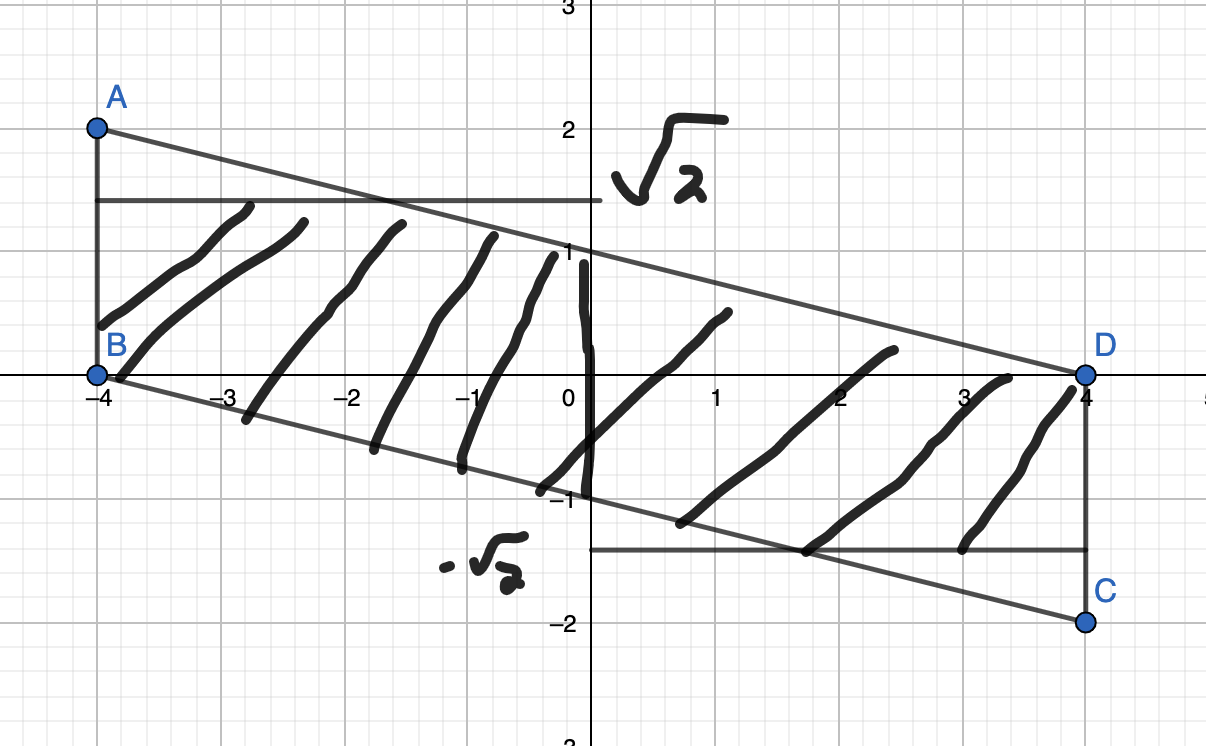
\includegraphics[scale=0.4]{5.png}
\end{center}
\[
P(|y_q| \leq \sqrt{2}) = 1 - 2 \cdot \frac{(2-\sqrt{2})^2}{8} = \frac{1}{2} (2 \sqrt{2} - 1)
\]
\[
P(x_q \leq 0)  \cdot P(|y_q| \leq \sqrt{2})  =  \frac{1}{4} (2 \sqrt{2} - 1)
\]
\[
P(x_q \leq 0\;  \cap  \; |y_q| \leq \sqrt{2}) = P(\text{аналогичная вероятность из пункта b}) = \frac{1}{4} \left(2\sqrt{2} - 1\right)
\]
\[
P(x_q \leq 0)  \cdot P(|y_q| \leq \sqrt{2})  = P(x_q \leq 0\;  \cap  \; |y_q| \leq \sqrt{2})
\]
$\rightarrow$ \textbf{события НЕзависимы}
\clearpage
\section*{Номер 3}
\begin{center}
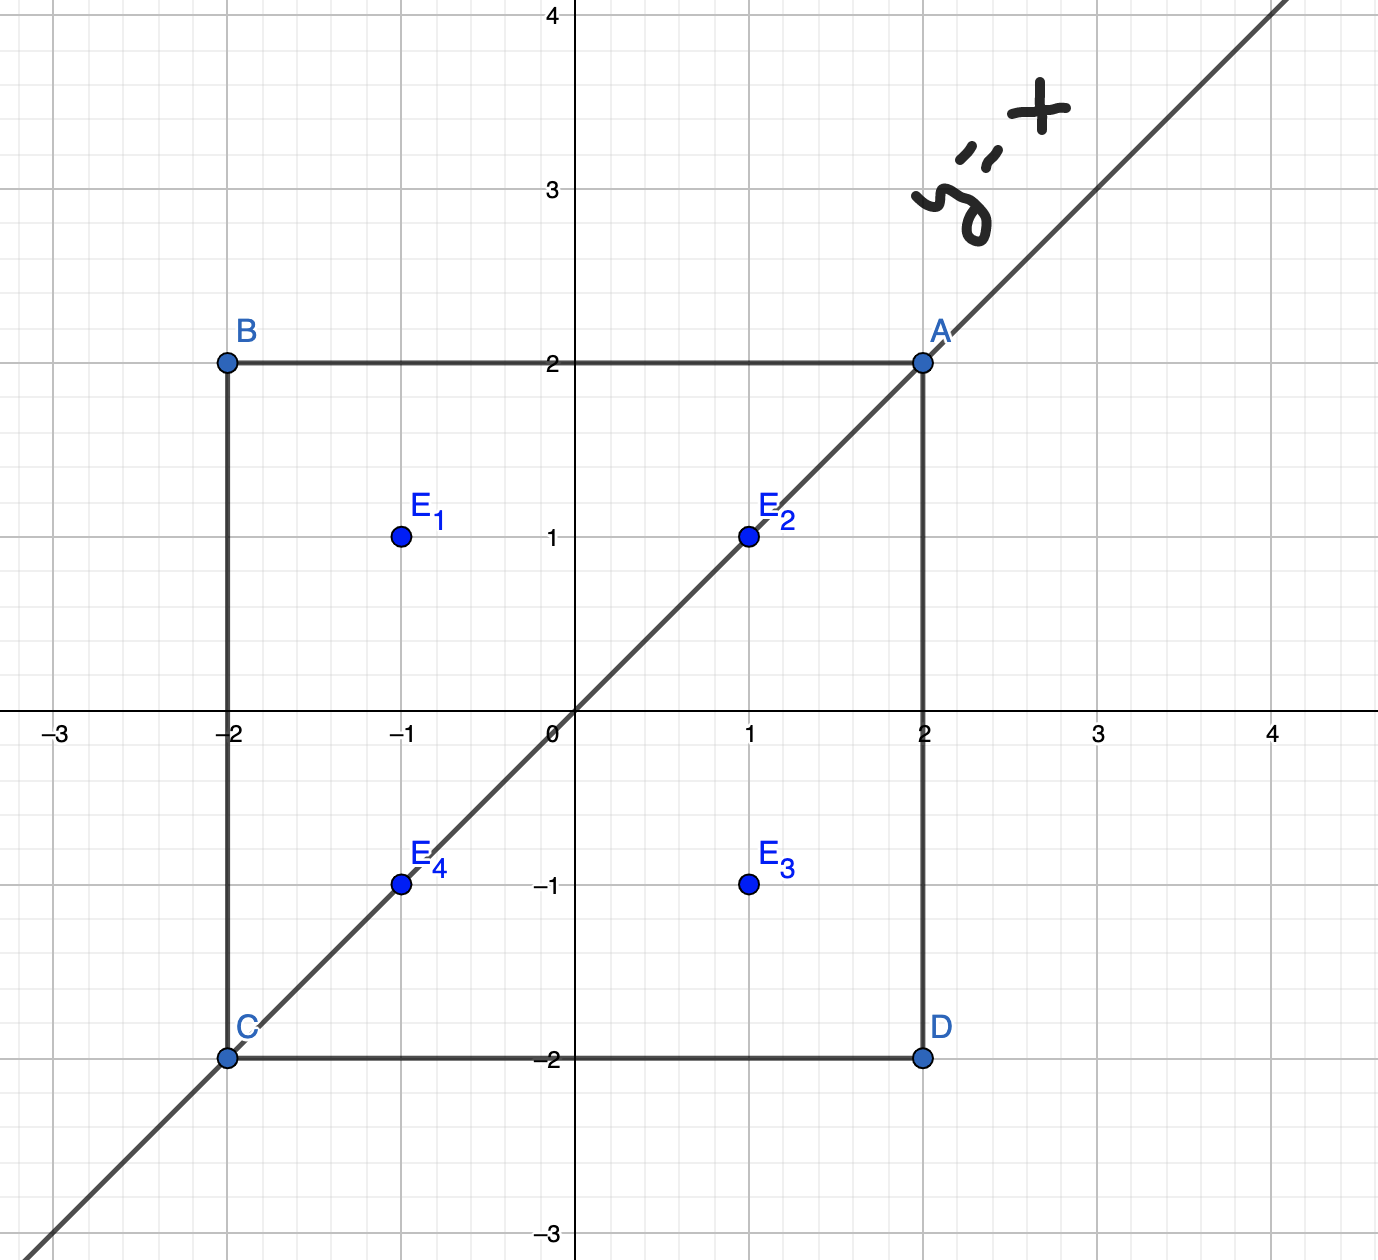
\includegraphics[scale=0.2]{6.png}
\end{center}
\subsection*{a)$P(x_Q \leq y_Q | K = k) \; \forall \; k \in \{0, \ldots 6\}$}
Ну собственно считаем:
\\\\\
При $K = 1, 2, 4$ попадет в точки $E_1, E_2, E_4$ соотвественно ну и в треугольник $ABC$, при $ K = 3$ попадет в $E_3$  и не попадет в треугольник $ABC$

\[
P(x_Q \leq y_Q | K = 1) = 1
\]
\[
P(x_Q \leq y_Q| K = 2) = 1
\]
\[
P(x_Q \leq y_Q | K = 3) = 0
\]
\[
P(x_Q\leq y_Q| K = 4) = 1
\]
При $K = 5$ попадем в случайную точку квадрата, а нам подходит ровно его верхняя половина
\[
P(x_Q\leq y_Q | K = 5) = \frac{1}{2}
\]
При $K = 6$  попадем в случайную точку отрезка $E_1E_2$, любая из точек этого отрезка будет в $ABC$
\[
P(x_Q \leq y_Q | K = 6) = 1
\]
\section*{b) $P(x_Q \leq y_Q), P(x_Q < y_Q)$}
По формуле полной вероятности:
\[
P(x_Q \leq y_Q) = \sum_{k = 1}^6 P(x_Q \leq y_Q | K = k) \cdot P(K = k) = \frac{1}{6} \cdot \sum_{k = 1}^6 P(x_Q \leq y_Q | K = k) =
\]
\[
=
 \frac{1}{6} \cdot (1 + 1 + 0 + 1 + \frac12 + 1) =  \frac34
\]
Для $x_Q< y_Q $ нужно всего лишь исключить случаи попадания в крайние точки ($E_2$ и $E_3$), поэтому вероятности при $K = 2, K = 3$, будут равны нулю, вероятность при $K = 6$ не меняется, т.к у нас отрезок, получаем:
\[
P(x_Q < y_Q) = \sum_{k = 1}^6 P(x_Q < y_Q | K = k) \cdot P(K = k) = \frac{1}{6} \cdot \sum_{k = 1}^6 P(x_Q < y_Q | K = k) =
\]
\[
=
 \frac{1}{6} \cdot (1 + 0+ 0 + 0 + \frac12 + 1) =  \frac{5}{12}
\]
\end{document}
